\subsection{Modellspezifisch: Neuronale Netze}
Folgendes Unterkapitel beschäftigt sich mit solchen Methoden, welche sich auf neuronale Netze anwenden lassen.
\subsubsection{Layer-wise Relevance Propagation}
Layer-wise Relevance Propagation (LRP) wurde erstmals von \cite{bach2015pixel} vorgestellt und zeigt bei neuronalen Netzen die Relevanz eines Eingabewertes für die Ausgabe. \textcite{bach2015pixel} illustrieren dies in ihrem Paper sehr gut anhand eines Klassifikationsalgorithmus (CNN), welcher Bildern eine Klasse zuweist. Ein bestimmter Pixel ist hier die Eingabe und ist auf eine gewisse Weise für die Vorhersage verantwortlich. Um herauszufinden welche Pixel eines Bildes sich besonders auf die Vorhersage auswirken, wir im Rahmen der LRP-Methode ein Relevanzwert für jedes Neuron in jedem Layer berechnet, indem rückwärts durch das neuronale Netz gegangen wird. Somit wird sich in verkehrter Reihenfolge dem Input angenähert und die relevanten Pixel werden sichtbar. Dies nennen die Autoren \enquote{pixel-wise decomposition} \cite{bach2015pixel}. \textcite{bach2015pixel} stellen folgende Möglichkeit zur Berechnung der Relevanzwerte vor:
%Wie berechnet man nun die Scores? Man hat nun R14(erstes(und gleichzeitig einziges) Neuron im vierten (letzten) Layer), das hat z.B. einen Score von 0,8, dass es eine Katze ist - das ist unser erster Relevanz-Wert. Die Relevanz rechnet man nun so aus (Beweis siehe Orignalpaper): Relevanz ist R für das Neuron i, l ist der Layer:
\begin{equation}
    R_{i}^{(l)} = \sum_{i} \frac{z_{ij}}{\sum_{i'}z_{i'j}}R_{j}^{l+1} \text{wobei gilt:}\: z_{ij}=x_{i}^{(l)}w_{ij}^{(l,l+1)}
\end{equation}
$l+1$ sei hier der letzte Layer, mit dem gestartet wird und somit wird von hinten für jedes Neuron $j$ im Layer $l+1$ die Aktivierung berechnet. Diese Aktivierung ergibt sich dadurch, inwiefern sich ein Neuron $i$ im Vergleich zu den anderen Neuronen in dem Layer $l$ auswirkt. So werden die Gewichte mit dem Input $x$ mutlipliziert, welche sich jeweils in den nächsten Layer übertragen. Die Aktivierung gibt Aufschluss darüber, wie relevant ein Neuron jeweils für den nachfolgenden Layer (und somit auf den endgültigen Output) war. Ist dies für alle Layer geschehen, wird der ursprüngliche Input, also die Pixel des Bildes erreicht. Diese lassen sich dann visualisieren.

%Für die Anwendung von LRP kann eine Bibliothek unterstützen %\footnote{https://github.com/sebastian-lapuschkin/lrp_toolbox}.
\subsubsection{Saliency Maps}
Saliency Maps basieren auf einem ähnlichen Prinzip wie die LRP-Methode und lassen sich auch auf Bildklassifikation anwenden. Hier wird auch gezeigt, welche Teile eines Bildes releavant für die Vorhersage waren und es wird auf die innere Struktur des Netzwerkes zurückgegriffen \cite{Gianfagna.2021}.
Saliency Maps wurden zuerst vorgestellt von \cite{simonyan2013deep} und basieren auf der Berechnung, der Gradienten, welche bei der Optimierung der Verlustfunktion von neuronalen Netzen zum Einsatz kommen. Konkret helfen Gradienten dabei die Verlustfunktionsparameter zu optimieren, in dem vorgegeben wird, wie weit sich auf einer Funktion bewegt werden muss \cite{molnar2022}.

Nach \textcite{simonyan2013deep} gibt es hier ein Bild $I_{0}$ und eine Klasse $c$. Daneben existiert eine Klass-Score-Funktion $S_{c}(I)$. Ziel ist es, die Pixel anhand ihres Einflusses auf den Score $S_{c}(I)$ zu ordnen. Dieser Score ist zumeist in CNNs nicht linerar berechenbar, lässt sich jedoch annähern (mithilfe einer Taylor Series Expansion):
\begin{equation}
    S_{c}(I) \approx w^{T}I+b
\end{equation}
Analog zum Grundlagenkapitel sei hier b der Bias und $W$ sind die Gewichte. Die Saliency Map lässt sich für ein Merkmal $j$ wie folgt bestimmen \cite{kamath2021explainable}: 
\begin{equation}
    M_{j} = |w_{j}|
\end{equation}

Ein Beispiel für eine Saliency Map ist in Abbildung \ref{Fig:Saliency_Map_Beispiel} dargestellt.
Ein Vorteil dieser XAI-Methode besteht in ihrer leichten Berechnung und dass keine weiteren Annotationen zur Erklärung eingeführt werden müssen \cite{kamath2021explainable}. \textcite{Gianfagna.2021} schreiben jedoch, dass diese Art der Darstellung für Menschen nicht besonders hilfreich ist, da wenig erkannt werden kann. Daneben besteht ein Nachteil, welcher sich durch die Score-Funktion ergibt. Ist diese nicht ableitbar, lässt sich kein geeigneter Score ermitteln, was z.B. für die ReLu-Funktion gilt \cite{shrikumar2017learning}. DeconvNet von \cite{zeiler2014visualizing} ist ein ähnlicher Ansatz, welcher das Problem mit der ReLU-Function löst. Grundsätzlich können jedoch auch LIME oder SHAP für das Erstellen von Saliency-Maps genutzt werden \cite{molnar2022}.
\begin{figure}[h]
    \centering
    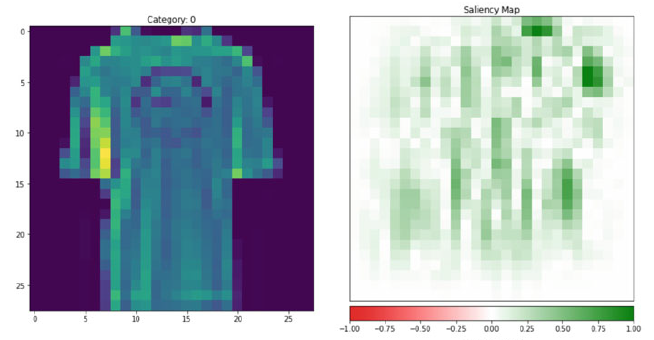
\includegraphics[scale=0.45]{pic/MA-Bilder/Literaturrecherche/Saliency-Map-Beispiel.PNG}
    \caption{Beispiel für Saliency Map, entnommen aus: \cite{kamath2021explainable}}
    \label{Fig:Saliency_Map_Beispiel}
\end{figure}

\subsubsection{TCAV}
TCAV steht für \enquote{Testing with Concept Activation Vectors} und wurde von \textcite{kim2018interpretability} vorgestellt. Diese Methode konzentriert sich darauf, mithilfe von Konzepten die Funktionsweise von neuronalen Netzen Menschen näher zu bringen. Nach \textcite{kim2018interpretability} bringen viele andere XAI-Methoden den Nachteil mit sich, dass die Fokussierung auf Merkmale schlecht für Nutzer zu interpretieren ist. Merkmale liegen häufig in niedriger Abstraktionsebene vor, aber Menschen denken nicht auf niedriger, sondern auf hoher Abstraktionsebene - in Konzepten. 
%Motiviert wird die TCAV-Methode durch eine Schwäche von Saliency Maps und den sogenannten \enquote{Confirmation Bias}. Sie untersuchten verschiedene Arten von Saliency Maps und fanden heraus, dass selbst, nachdem sie das Modell so modifizierten, dass dieses zufällige Vorhersagen traf, die Maps sich kaum veränderten. %Hier kommt der \enquote{Confirmation Bias} ins Spiel. Wenn Menschen etwas bestimmtes erwarten, z.B. das ein Bild einer Katze so erklärt wird, dass die Umrisse von Katzenohren hervorgehoben werden, vertrauen sie dieser Erklärung durch eine Saliency Map, selbst dann, wenn dies nicht durch das Modell erkannt wird. 
%Ein Problem kann sein, dass Pixel genutzt wurden und nciht high-Level (Menschen denken nciht in Pixel)
%Sie wollen high-Level-Konzepte nutzen. Sie sieht Interpretierbarkeit als Optimisierungsproblem, man muss eine Erklärung E finden, so dass Q maximiert ist. Das Q kann eine subjektive Measures sein, sodas man Menschen fragt, aber auch 
%\begin{equation}
%    \underset{E}{argmax} Q(E|?)
%\end{equation}

%Sie sagt auch ncoh, wie man das gut prüfen kann, ob eine Erklärung gut war: gib Menschen Task, für die Verständnis über das Modell wichtig ist --> wenn die die gut können, bedeutet dass, dass sie das Modell verstanden haben

%kommt nur im Youtube-Video vor:
%Modell Matters--> also linear ist einfacher als krumme komische Geraden
%Data Matters --> wenn die Daten voll gut linear abtrennbar sind, weil sie so sind, ist es einfach, aber wenn die überall drin liegen und die lineare Gerade dadurch sich nur annähert, ist doof, Daten sind halt nicht so
%Empfänger matters: wenn ich es Nutzern erläre oder Leuten, die es weiterentwickeln wollen, stellen die andere fragen
%Task matters: lokal vs. global, eibfach vs. komplex (dafür genauer), Domäne (einfach oder leicht)
 
%TCVA: ist eine Post-Methode
Die TCVA-Methode kann genutzt werden, um auf hoher Abstraktionsebene zu testen, ob ein bestimmtes Konzept in die Vorhersage des Algorithmus miteinfloss. Dies ist sogar dann möglich, wenn dieses Konzept nicht Teil des Trainingsdatensatzes war. Illustriert wird die Fuktionweise in Abbildung \ref{Fig:TCAV} \cite{kim2018interpretability}.

\begin{figure}[h]
    \centering
    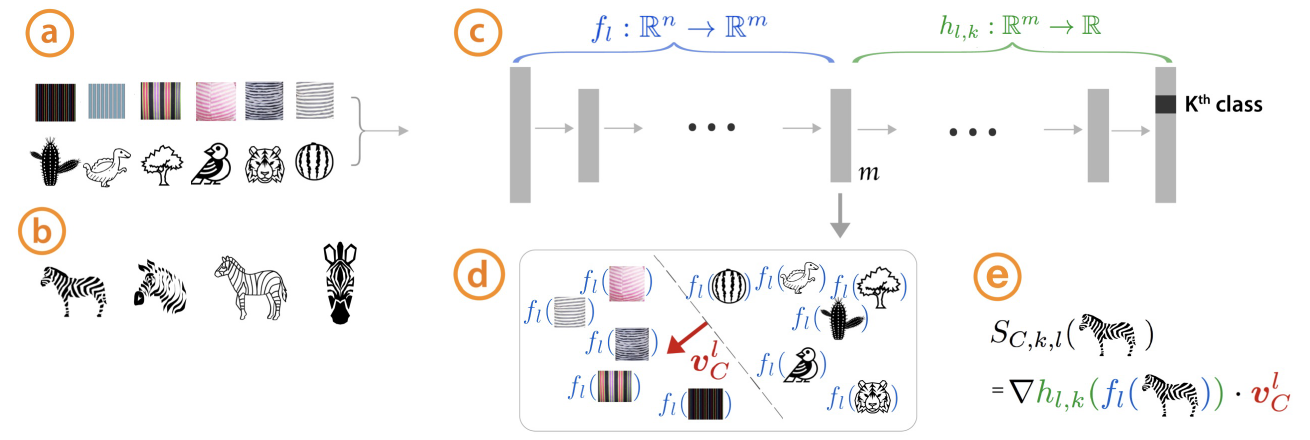
\includegraphics[scale=0.45]{pic/MA-Bilder/Literaturrecherche/TCAV.PNG}
    \caption{Funktionsweise von TCAV, entnommen aus: \cite{kim2018interpretability}}
    \label{Fig:TCAV}
\end{figure}
Als Beispiel ist hier ein neuronales Netz, welches Bilder klassifziert und ausgibt, ob sich auf dem Bild ein Zebra befand. Was nun von Interesse sein kann, ist die Frage, ob das Konzept \emph{Streifen} mit in die Bestimmung der Vorhersage einfloss. Konzepte lassen sich als Vektoren (CVA: Contept Activation Vector) definieren. Um einen solchen Vektor zu bilden, sind zunächst Beispiele von Nöten, z.B. Bilder von Streifen. Daneben werden noch andere, zufällige Bilder benötigt. Eine weitere Voraussetzung für das Durchführen der TCAV-Methode ist der Zugang zum Netzwerk und seinen Aktivierungen. Zu Beginn werden alle Beispiele (solche mit Streifen und solche ohne) durch das Netzwerk geleitet und die Aktivierungen gesammelt. Daraufhin wird ein linearer Klassifikationsalgorithmus trainiert, welcher die beiden Klassen voneinander abgrenzt. Der CVA steht nun orthogonal auf der durch den linearen Klassifzierungsalgorithmus erstellten Entscheidungsgrenze und zeigt auf die Bilder, welche Streifen enthielten. Nun kann mittels des Vektors das Konzept getestet werden.
\todo{Hier fehlt noch, wie das Testen an sich funktioniert}

%Man betrachtet Konzept zu CAV: Man nimmt jetzt das Konzept (den Vektor) und das Bild (das Zebra) und verändert das Bild so, dass man mehr oder weniger von dem Konzept nimmt und schaut, ob siech die Prediciton-Wahrscheinlichkeit für Klasse Zebra verändert. Wenn es sich gar nicht verändert, ist das Konzept nicht wichtig
%Man nimmt jetzt viele Zebra-Bilder und schaut wieviele positiv directional für CAV(Streifen) ausgaben

%Problem mit den Images, einige waren random und daher fragt sich KIM: Hat mein CAV nur hohe Empfindlichkeit durch Zufall geliefert? --> das kann man überprüfen, indem man ganz viele Random Images merhmals mit den Streifen vergleicht und hierfür mehrer TCAVs macht %todo weglassen oder verstehen :D
%Wenn das Konzept wirklich sinnvoll ist, dann der TCAV-Score auch immer ähnlich sein
%Vorteil: Nutzer kann mit eigenen Konzepten ankommen und braucht nix über ML zu wissen

%\cite{molnar2022}Methode kann globale erklärungen über Konzepte liefern
%\cite{kim2018interpretability} haben Methode vor allem auf Bildern angewendet, und es ist halt schwierig die Konzepte automatisch zu identifzieren, dafür braucht es halt Menschen

\todo[inline]{Ich würde noch die zwei unvollständigen Kapitel fertig schreiben und dann noch die Methode DeepLift, Neural Shrubs und etwas zu Feature Interaktionen schreiben}